\section{Energia}

A solução de energia do projeto consiste no dimensionamento de baterias que atendam às especificações e requisitos do sistema, tanto dos dispositivos eletrônicos quanto do sistema de ignição e lançamento. Além disso, será projetado um carregador de bateria para tornar contínuo o uso do equipamento.

Para dimensionar o consumo do sistema, foi observado o gasto energético dos componentes eletrônicos, levando em conta que o projeto precisa de uma autonomia de, no mínimo, duas horas de uso sem a possibilidade de ter como fonte de energia a rede elétrica.

Anteriormente, ao dimensionar o sistema de alimentação do projeto, foi definido que seria utilizada apenas uma bateria que alimentasse todos os componentes. Porém, ao avaliar melhor as necessidades do projeto, em especial a distância de segurança (500m) entre o usuário e a base de lançamento do foguete, optou-se por dimensionar dois sistemas, de forma a eliminar a utilização de cabos para alimentar os componentes que precisariam estar na base.

A utilização de cabos entre a base e o sistema de controle, além de não ser viável do ponto de vista do usuário, também provocaria impactos a serem considerados no projeto, como a queda de tensão atrelada a um cabo de grande extensão como o que seria necessário.

Sendo assim, para aumentar a qualidade e melhorar a usabilidade do produto, foi definido que o projeto será composto por dois sistemas: o sistema de controle e o sistema da base. Cada sistema será alimentado eletricamente de forma individual. Os dois sistemas estarão interligados por telemetria, conforme descrito na solução de eletrônica, e serão controlados pelo usuário, que utilizará o sistema de controle (maleta) a uma distância segura da base de lançamento.

\subsection{Ignição}
\label{sec:ignição}

Para dimensionar o sistema de alimentação elétrica do projeto, é necessário realizar o dimensionamento do consumo de potência do ignitor, que faz parte do sistema da base de lançamento. O tipo de ignitor utilizado pela \textit{{Equipe Capital Rocket Team}} é o fio de Níquel Cromo (Ni-Cr), os cálculos foram realizados com base nesse tipo de ignitor.

Para o ignitor de Níquel Cromo foi considerado o diâmetro de $0,8 mm^2$ e temperatura de ignição de 300ºC, a \textit{Capital Rocket Team} não dispunha dessas informações, mas esses foram os parâmetros mais comuns encontrados para esse tipo de sistema \cite{edufer2020}.  

No site do fabricante \cite{ignitor}, há uma tabela que permite, com a entrada desses dados, obter a resistência (em Ohm/m). A partir desse dado, utilizando a primeira Lei de Ohm, com o valor de tensão fornecido pela bateria (12V) será calculada a corrente consumida pelo ignitor.

A resistência obtida por meio da tabela do fabricante é de 2,23 Ohms/m, considerando um enrolamento de 1m, a resistência do ignitor é 2,23 Ohms. A corrente pode ser descrita de acordo com a primeira Lei de Ohm:

\begin{center}
\begin{equation}
 I = \frac{V} {R} 
 \end{equation}
 
 \begin{equation}
 I = \frac{12} {0,23}
 \end{equation}
 
 \begin{equation}
 I = 5,38 A
\end{equation}
\end{center}

Com o valor da corrente obtido e com base na relação entre corrente, tensão e potência, pode ser calculada a potência consumida.

\begin{center}
\begin{equation}\label{m}
	P = I \times V 
    \end{equation}
    
 \begin{equation}
  P =  5,38 \times 12 
  \end{equation}
  
  \begin{equation}
  P = 64,56 W 
\end{equation}
\end{center}

O ignitor será utilizado somente uma vez a cada lançamento, e apenas para o momento de ignição do foguete. Para fins de segurança, de forma a garantir a autonomia do sistema, será adotado o tempo de utilização de 15 minutos.

\subsection{Consumo dos sistemas}

Como dito anteriormente o projeto é separado por dois sistemas a maleta e a base de lançamento. Nas tabelas \ref{tab:consumo1} e \ref{tab:consumo2} é apresentado o consumo dos principais componentes elétricos e eletrônicos de cada um dos dois sistemas e uma estimativa do período que cada componente será utilizado durante um lançamento. 

\begin{center}
\begin{table}[H]
\centering
\begin{tabular}{ |m{4cm}|m{2cm}|m{2cm}|m{2cm}|m{3cm}|} 
\hline
\textbf{Componentes}&\textbf{Tensão} & \textbf{Corrente}& \textbf{Potência} & \textbf{Tempo de Utilização}\\ 
 \hline
 Tela & 12V & 1A & 12W & 2h30m\\
  \hline
Jetson Nano Developer Kit & 5V & 2A & 10W & 2h30m\\
  \hline
 Teclado e botões & 5V & 250 mA & 1,25W & 2h30m\\ 
  \hline
 Módulo LORA - maleta & 5V & 500mA & 2,5W &2h30m\\ 
 \hline
 
 \hline
\end{tabular}
\caption{Consumo elétrico dos componentes da maleta.}
\label{tab:consumo1}
\end{table}
\end{center}

Com base na tabela \ref{tab:consumo1}, o somatório de potências do sistema é de 25,75W. Será utilizado o valor de 30 W por segurança. O lançamento de um foguete tem duração média de 2 horas, o valor utilizado será de 2 horas e 30 minutos, por segurança.

Sendo assim, o somatório da potência é multiplicado pelo tempo em horas.

\begin{equation}
    30W \times 2,5h = 75 Wh
\end{equation}

\begin{center}
\begin{table}[H]
\centering
\begin{tabular}{ |m{4cm}|m{2cm}|m{2cm}|m{2cm}|m{3cm}|} 
\hline
\textbf{ Componentes }&\textbf{ Tensão} & \textbf{Corrente }& \textbf{Potência} & \textbf{Tempo de Utilização}\\ 
 \hline
 Módulo LORA - base & 5V & 500mA & 2,5W & 2h5m\\ 
 \hline
 Ignitor (Ni-Cr) & 12V & 5,38A & 64,56W & 15m \\
 \hline
 Atuadores (3x) & 12V & 3.9A & 46,8W & 15m \\ 
 \hline
\end{tabular}
\caption{Consumo elétrico dos componentes da base de lançamento.}
\label{tab:consumo2}
\end{table}
\end{center}

Para a alimentação dos componentes, vão ser utilizadas tensões contínuas de 5 V e 12 V. A bateria a ser utilizada será de 12V, já que a maior tensão dentre os equipamentos.

Com base na tabela \ref{tab:consumo2}, o somatório de potências do sistema é de 113,86W; porém, o valor utilizado de 2 horas e 30 minutos será usado apenas para o módulo, o ignitor e os três atuadores funcionam apenas nos primeiros minutos do lançamento. Por isso para calcular a potência destes será usado o tempo de 15 minutos.

Para o módulo:
\begin{equation}
    2,5W \times 2,5h = 6,25 Wh
\end{equation}

Para ignitor e atuadores:

\begin{equation}
    111,36W \times 0,25h = 27,84 Wh
\end{equation}

A potência total consumida pela base é :

\begin{equation}
    6,25Wh + 27,84Wh = 34,09 Wh
\end{equation}

Essa será a energia necessária consumida para a autonomia especificada. Por segurança será considerado o valor de 40 Wh.
Pela Lei de Ohm temos:

\begin{equation}
   I =  \frac{P}{V}
   \end{equation}
   
   \begin{equation}
      I =  \frac{34,09}{12}
   \end{equation}
   
  \begin{equation}   
   I = 3,33 Ah
 \end{equation}

\subsection{Baterias}

As duas baterias serão de 12V, já que esta é a maior tensão dentre todos os equipamentos nos dois sistemas.

Dentre os tipos mais comuns de baterias no mercado, estão as de chumbo-ácido e de íons de lítio. 

A bateria de chumbo-ácido é a mais comum, é comercializada há mais tempo e requer pouca manutenção. Esse modelo não possui efeito memória, que diminui a capacidade de carga. Porém, o chumbo, além de ser tóxico, possui baixa densidade de energia,  o que limita sua aplicação a sistemas portáteis leves \cite{baterias}.

As baterias de íons de lítio tem como componente principal o lítio, que é um metal leve e com grande potencial eletroquímico, o que proporciona uma grande densidade de energia. Esse tipo de bateria também não possui efeito memória, importante em sistemas que sofrerão cargas e descargas frequentemente. Porém, essa tecnologia é mais recente, e o custo das baterias de íons de lítio é mais elevado \cite{baterias}. 

\subsubsection{Sistema de controle - maleta} 

Para a bateria do sistema de controle, em formato de maleta, buscou-se no mercado o tipo de bateria mais compacto possível de forma a atender a carga dimensionada, o modelo mais adequado encontrado foi o modelo de baterias de notebook, que é de íons de lítio. 

De acordo com o dimensionamento, a potência consumida é de 75Wh. Por questões de segurança será considerada uma descarga máxima de 80\%, sendo assim a capacidade da bateria será:

Capacidade em Wh
\begin{equation}
    75/0,8 = 93,75 Wh
\end{equation}

A capacidade necessária para esse sistema é de 93,75 Wh. Foi selecionada uma bateria da fabricante Dell, de 9 células e capacidade de 97 Wh, com as características a seguir:

Peso: 508,02 g

Dimensões

- Profundidade: 71,79 mm 

- Altura: 20,00 mm 

- Largura: 214,00 mm  


Na Figura \ref{fig:bateriamaleta} é apresentada a bateria selecionada para a maleta.

\begin{figure}[!h]
	\centering
		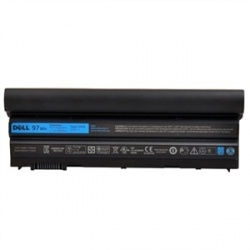
\includegraphics[keepaspectratio=true,scale=1]{figuras/bateria_maleta.jpg}
	\caption{Bateria selecionada para o sistema de controle. Fonte: \cite{figura_bateria_maleta}} 
	\label{fig:bateriamaleta}
	\end{figure}

\subsubsection{Sistema da base de lançamento} 

A capacidade calculada para o sistema da base de lançamento foi de 3,33 Ah. De acordo com o fabricante a capacidade da bateria deve ser mantida entre 50\% - 60\%, por segurança e de forma a prolongar a vida útil do equipamento. Considerando então uma descarga máxima de 40\% a capacidade da bateria será:

Capacidade em Ah
\begin{equation}
     3,33/0,4 = 8,33 Ah
\end{equation}

A capacidade necessária para esse sistema é de 8,33 Ah, a bateria selecionada deve ter capacidade de 9 a 10 Ah. Como mencionado anteriormente, as baterias mais comuns no mercado são de chumbo-ácido e de lítio. Dessa forma, buscou-se fabricantes que possuíssem os dois tipos de bateria, com a capacidade necessária para o sistema, para realizar uma comparação e selecionar a mais adequada.

Durante as pesquisas encontrou-se informações mais completas do fabricante \textit{Unipower}, esse fabricante possui um modelo de bateria de chumbo-ácido de 12V e 9Ah e um modelo de lítio, de 12V e 10Ah. Ambas as baterias possuem as mesmas dimensões $(100mm \times 151mm \times 65mm)$, porém, a bateria de chumbo-ácido pesa 2,5 kg enquanto a bateria de lítio pesa 1,5 kg. Como o sistema deve ser portátil é importante que ele seja o mais leve e compacto possível, dessa forma foi escolhido o modelo de lítio, que é mais leve e tem maior capacidade. O fabricante \textit{Unipower} trabalha com um tipo específico de baterias de íons de lítio, as baterias de lítio ferro fosfato.

A bateria selecionada é a Bateria Lítio Ferro Fosfato - LiFePO4, modelo UPLFP12-10.  Na Figura \ref{fig:bateriabase} é apresentada a bateria selecionada para a base de lançamento. 

\begin{figure}[!h]
	\centering
	\label{bateria_base}
		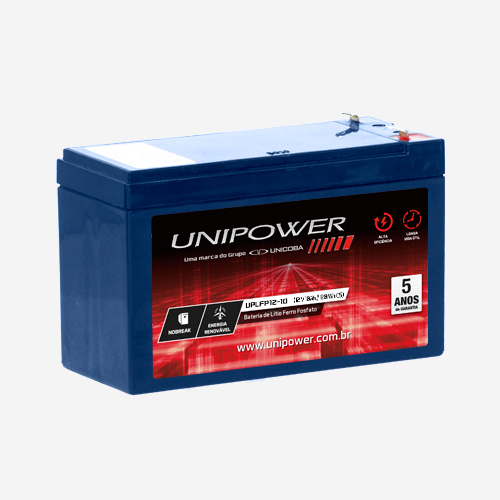
\includegraphics[keepaspectratio=true,scale=0.6]{figuras/bateria_base.jpg}
	\caption{Bateria selecionada para a base de lançamento. }
	{\footnotesize Fonte: \cite{datasheet_bateria}}
	\label{fig:bateriabase}
\end{figure}

\subsection{Regulador de tensão}

Como as fonte de tensão são de 12V, serão utilizados módulos “\textit{step down}” para regular as tensões direcionadas para alguns componentes do sistema. No projeto, será utilizado o módulo regulador de tensão modelo LM2596 apresentado na figura \ref{fig:regulador tensao}, pois este possui uma ampla faixa de tensões de entrada e pode ser regulado para uma tensão específica de saída com uma boa eficiência \cite{datasheet_regulador}.

A faixa de tensão utilizada será de 5V, de acordo com a necessidade de cada dispositivo eletrônico no sistema.

\begin{figure}[!h]
	\centering
	\label{regulador_tensão}
		\includegraphics[keepaspectratio=true,scale=1]{figuras/regulador_de_tensão.jpg}
	\caption{Regulador de tensão modelo LM2596.}
	\label{fig:regulador tensao}
\end{figure}

\subsection{Funcionamento do sistema de alimentação}

A partir da definição de todos os equipamentos é possível visualizar o funcionamento de cada sistema de alimentação.  

O diagrama em blocos do sistema de controle pode ser observado na Figura \ref{fig:blocosmaleta}.

\begin{figure}[!h]
	\centering
		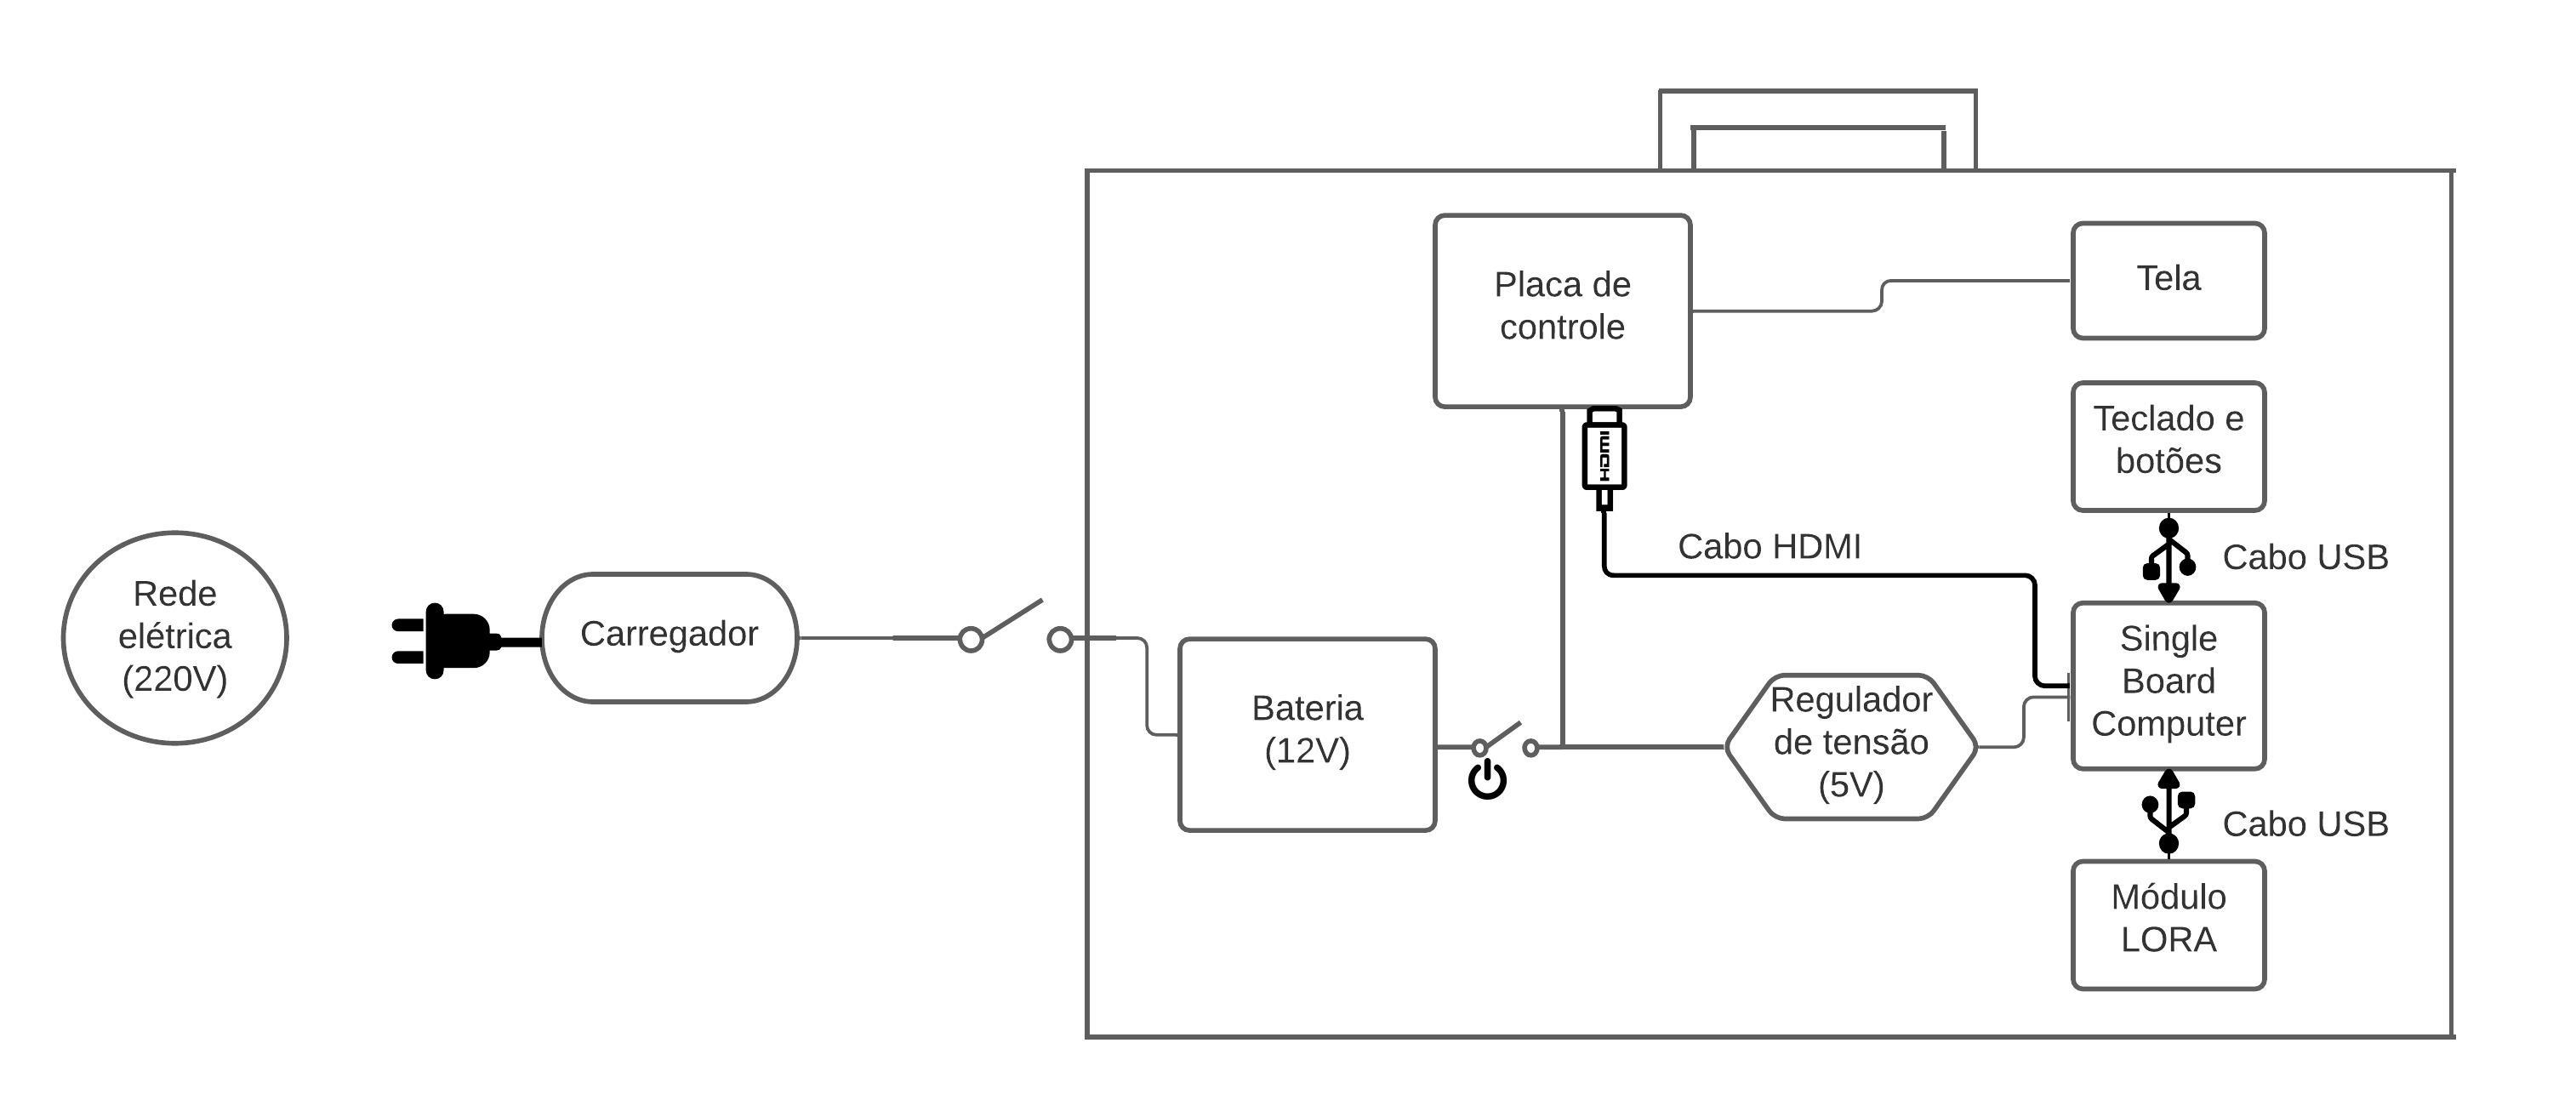
\includegraphics[keepaspectratio=true,scale=0.6]{figuras/blocos_maleta.jpeg}
	\caption{Diagrama em blocos do sistema de controle - maleta.}
	\label{fig:blocosmaleta}
\end{figure}

Nesse sistema a bateria alimenta diretamente a placa de controle da tela e o módulo regulador de tensão. Nesse ponto de alimentação está inserido um botão interruptor, de forma a ligar ou desligar o sistema como um todo.

O regulador de tensão, por sua vez, alimenta o \textit{Single Board Computer} que se conecta ao teclado e ao módulo LORA via cabo USB, além disso, o \textit{Single Board Computer} se conecta a placa de controle da tela via cabo HDMI. 

O diagrama em blocos do sistema da base de lançamento pode ser observado na Figura \ref{fig:blocos_base}.

\begin{figure}[!h]
	\centering
		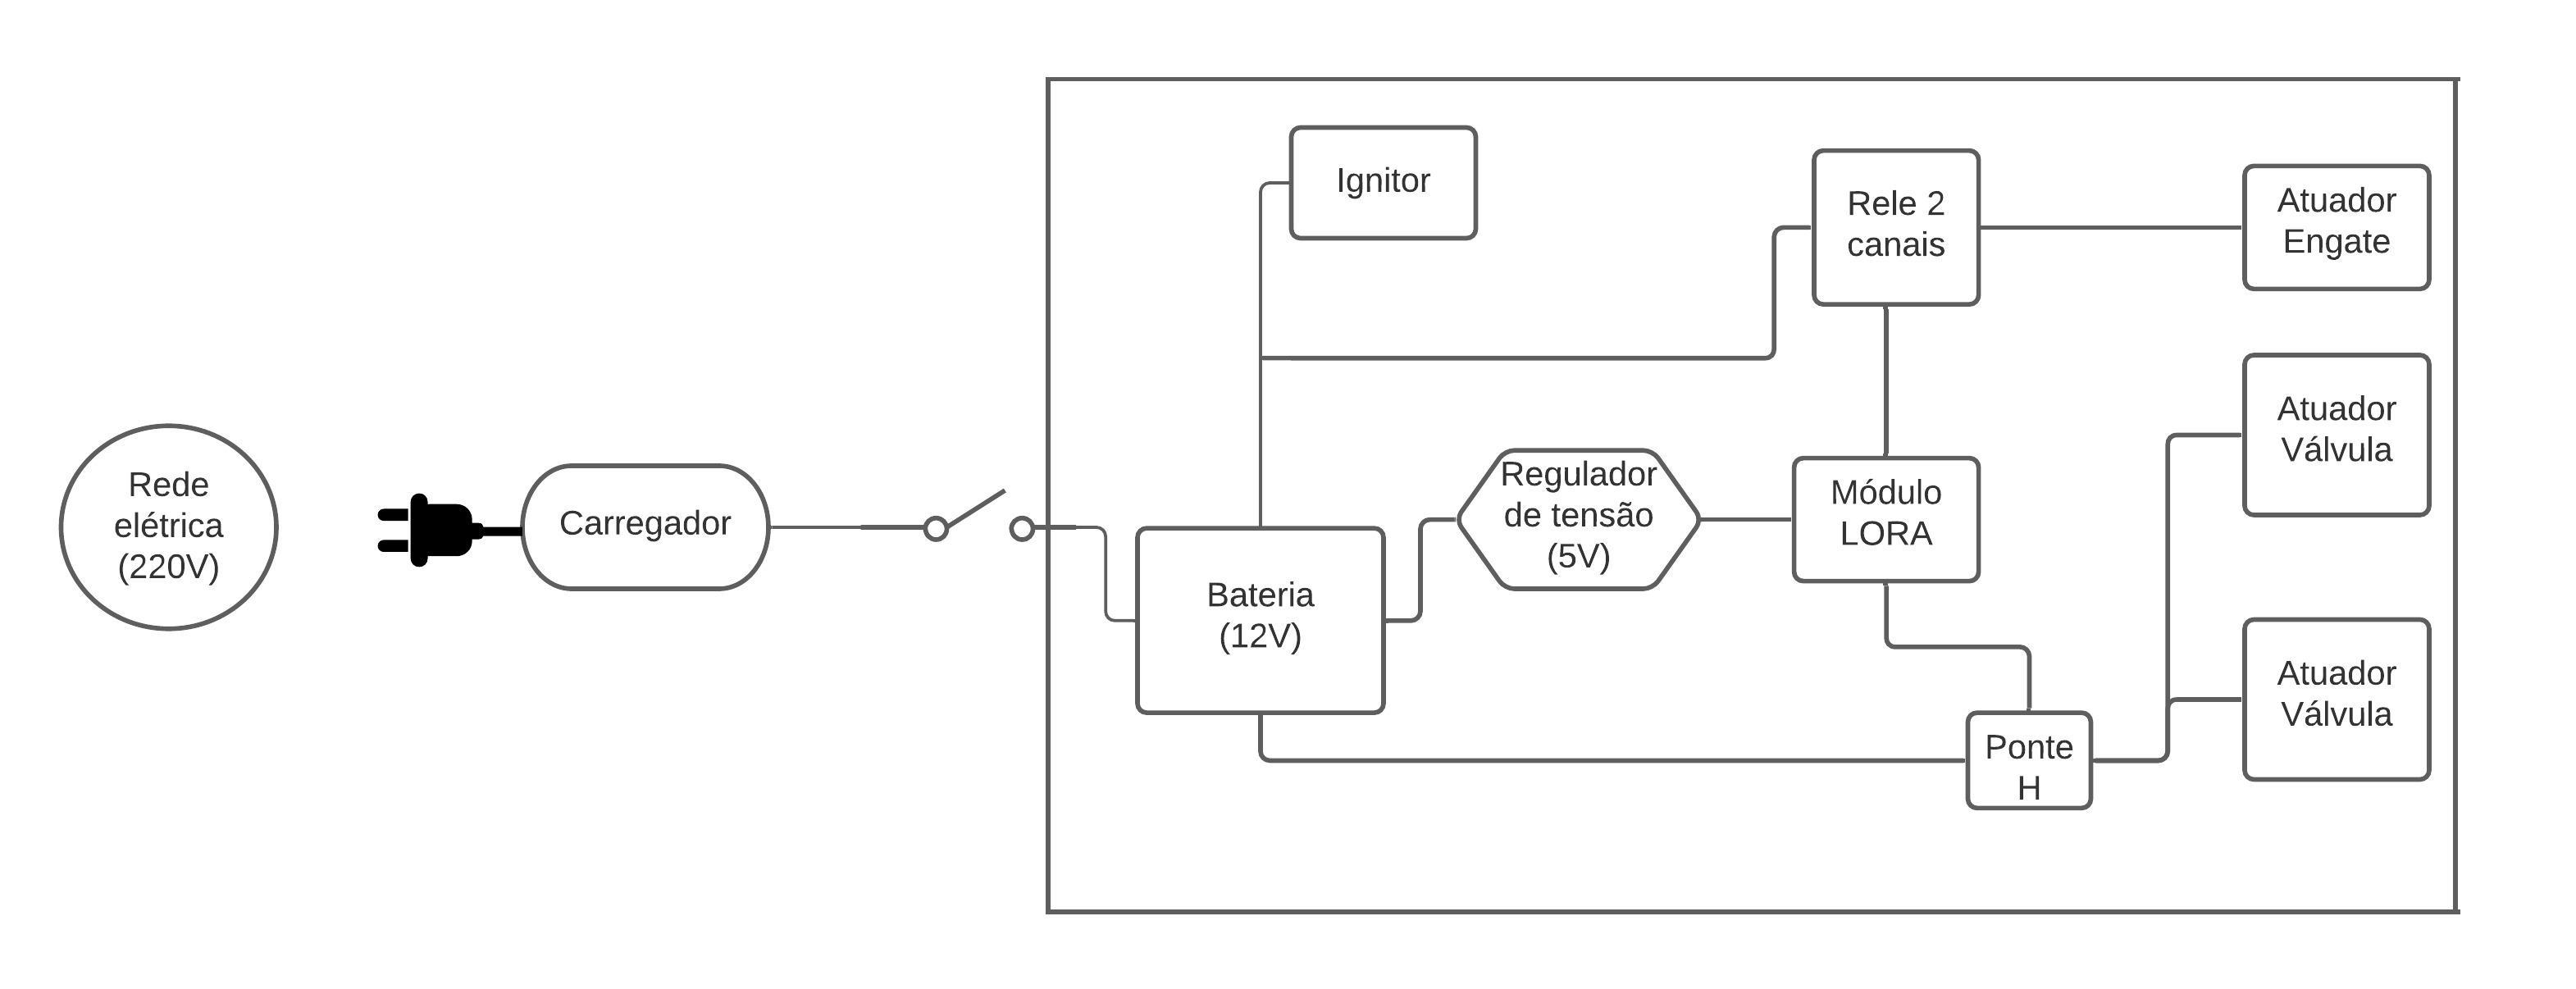
\includegraphics[keepaspectratio=true,scale=0.6]{figuras/blocos_base.jpeg}
	\caption{Diagrama em blocos da base de lançamento.}
	\label{fig:blocos_base}
\end{figure}

No sistema da base de lançamento a bateria alimenta diretamente o ignitor, o circuito ponte H, o módulo relé 2 canais e o módulo regulador de tensão. Nesse sistema, não foi inserido o botão liga/desliga, pois os componentes serão ativados por meio do sistema de controle.

Os atuadores das válvulas são alimentados por meio do circuito ponte H, o atuador do engate é alimentado por meio do relé 2 canais, o relé e o circuito ponte H estão conectados com o módulo LORA, que é alimentado por meio do módulo regulador de tensão.

É possível observar ainda, em ambos os sistemas, o esquema de carregamento da bateria, a conexão entre o carregador e a bateria está representada por um interruptor, pois essa conexão não é fixa, e será realizada apenas nos momentos de carregamento de cada bateria. A conexão será feita por meio de um conector \textit{Jack}, presente em cada uma das estruturas.

\subsection{Carregador de bateria}

A solução inicial para o sistema consistia em realizar o carregamento da bateria \textit{off grid}, ou seja, sem conexão com a rede elétrica, a partir do uso de placas fotovoltaicas. Porém, ao analisar as condições de operação do sistema, em especial o tempo de operação, que é previsto para no máximo 2 horas, concluiu-se que a solução mais adequada seria realizar o carregamento \textit{on grid}, conectado à rede elétrica, a partir de um carregador de bateria, a ser projetado.

Dessa forma, as baterias, tanto da maleta quanto da base, serão levada com carga completa até o local de lançamento, todo o sistema poderá ser alimentado a partir delas, e, ao retornar para um local com conexão à rede elétrica, as baterias poderão ser recarregadas, e o sistema estará pronto para o próximo uso.

Como as duas baterias são de Íon-Lítio, será projetado um único carregador que seja compatível com as especificações técnicas das duas baterias usadas no projeto, a tensão de saída deve ser no máximo de 14,6V e a corrente máxima de saída 10A.

\subsubsection{Fonte de Alimentação}

A fonte de alimentação será a  responsável por entregar a tensão e a corrente necessária para carregar as duas baterias do sistema, como o carregador será ligado à rede elétrica, foi projetado um circuito capaz de converter corrente alternada (rede elétrica) para corrente contínua (usada no projeto) e fazer a redução de tensão (no caso, de 220V para 30V). Para isso, foi inserido um transformador e um retificador de onda completa.

\textbf{Transformador}
    
Um transformador é constituído basicamente de dois enrolamentos onde o fluxo magnético, variável, produzido em um age sobre o outro. O enrolamento no qual a fonte é aplicada é o primário do transformador e o enrolamento onde a carga é conectada é o secundário \cite{transformadores}.

Para o projeto, deseja-se a utilização de um transformador de tensão (com \textit{center-tapped}), que será responsável por abaixar a tensão. Em nosso caso, a tensão de entrada será a tensão fornecida pela rede, que é de 220V alternada, e a tensão de saída será a tensão desejada para o funcionamento do projeto, que será de 30V, ainda alternada na saída do transformador.

\textbf{Retificador de onda completa}

Como a tensão na saída do transformador é alternada é necessário um retificador para torná-la contínua, o Retificador de onda completa consiste no uso de 2 diodos acoplados ao transformador que contenha \textit{center-tapped}, para garantir a retificação de onda completa. 

Os diodos são dispositivos eletrônicos que permitem a passagem de corrente elétrica em apenas um sentido. Eles só permitem a passagem de corrente elétrica quando esta é polarizada diretamente, ou seja, quando o polo positivo da fonte entra em contato com o polo positivo do diodo \cite{retificador}. No circuito, o diodo funciona de acordo com a figura \ref{fig:retificador}

\begin{figure}[!h]
	\centering
		\includegraphics[keepaspectratio=true,scale=0.5]{figuras/retificador_completo.JPG}
	\caption{Esquemático de um retificador de onda completa. Fonte: \cite{retificador}}
	\label{fig:retificador}
\end{figure}

\subsubsection{Circuito de carregamento}

O carregador de baterias de lítio íon é um dispositivo limitador de tensão similar ao carregador de baterias de chumbo-ácido. A diferença está em uma maior tensão por célula, uma tolerância de tensão menor e a ausência de carga de flutuação ou pulsante quando a carga completa é alcançada \cite{bateria_litio}.

O tempo de carga de todas as baterias de Lítio-Íon, quando carregadas a uma corrente inicial de 1 C, é de aproximadamente 3 horas. A bateria permanece fria durante a carga. A carga completa é alcançada depois que a tensão alcança o limiar de tensão superior e a corrente ter caído e se igualado a 3\% da corrente de carga nominal. Na figura \ref{fig:curvacarga}, é mostrada a curva de carga de uma bateria de Lítio íon.

\begin{figure}[!h]
	\centering
		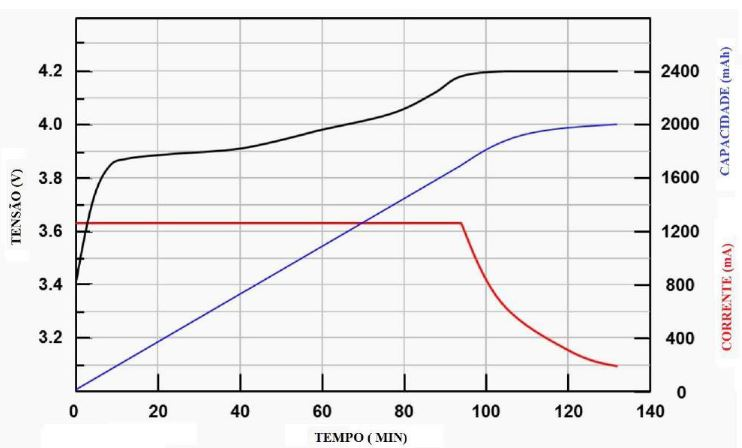
\includegraphics[keepaspectratio=true,scale=0.5]{figuras/Curva_carga.JPG}
	\caption{Curva de carga da bateria de Lítio íon. Fonte: \cite{bateria_litio}}
	\label{fig:curvacarga}
\end{figure}

Baterias de lítio íon são projetadas para operar seguramente dentro da sua tensão normal de operação, mas tornam-se cada vez mais instáveis se carregadas em voltagens maiores. Por esse motivo, é importante que haja circuitos internos de controle de tensão que interrompem a bateria em subtensão ou sobre tensão \cite{bateria_litio}.

Foi criado, usando o software Proteus, o circuito de carregamento das baterias (já inserida a fonte de alimentação). O apêndice \ref{diag_eletrico} contém o desenho do circuito criado. Nas figuras \ref{fig:bateriatensao} e \ref{fig:bateriacorrente} são apresentados os testes de simulação do circuito contendo as medições de tensão e corrente.

\begin{figure}[!h]
	\centering
		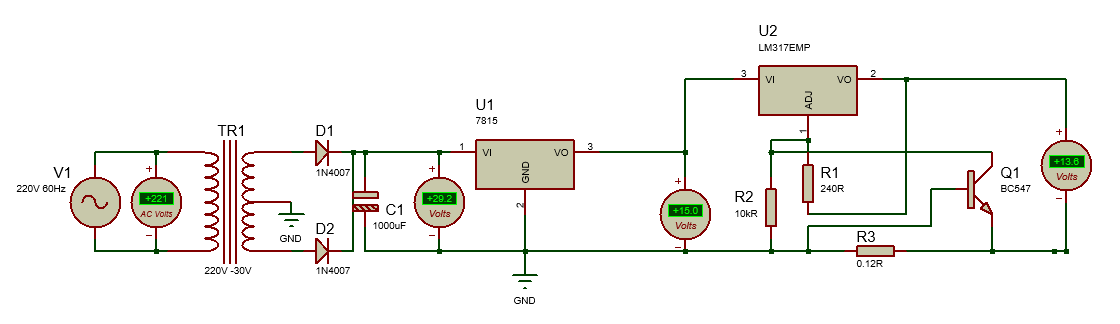
\includegraphics[keepaspectratio=true,scale=0.5]{figuras/Medição - Tensão.PNG}
	\caption{Medição de tensão no circuito carregador. Fonte: \cite{retificador}}
	\label{fig:bateriatensao}
\end{figure}

\begin{figure}[!h]
	\centering
		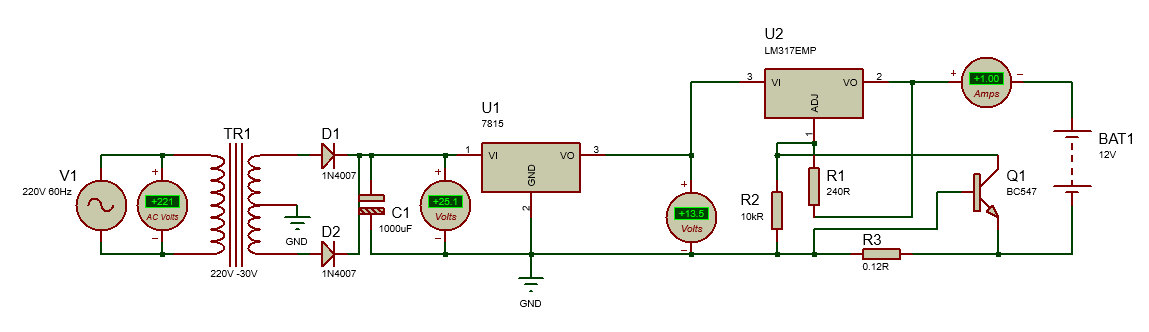
\includegraphics[keepaspectratio=true,scale=0.5]{figuras/Medição - Corrente.PNG}
	\caption{Medição de corrente no circuito carregador.}
	\label{fig:bateriacorrente}
\end{figure}

Observando as medições, é possível comprovar que, ao final do circuito, a bateria recebe uma tensão de 13.6V e uma corrente de 1A, capaz então de recarregá-la até 12V. O circuito de carregamento faz o controle da tensão para manter a carga, caso, depois de cheia, se a bateria perder a carga, o carregador reativa-se até ficar novamente com a carga completa. Desse modo, a bateria pode estar ligada de forma permanente ao carregador, mantendo a carga completa sem nenhum dano a bateria ou ao circuito.

\subsection{Dimensionamento dos condutores}

Para questões de dimensionamento dos condutores, o projeto será separado em três partes: carregador, maleta e base. Para determinar o diâmetro da seção transversal dos condutores utilizados no projeto, foi usada a norma NBR 5410/2004 \cite{NBR5410}. Segundo a norma, é preciso levar em conta dois parâmetros para decidir o diâmetro dos condutores: seção mínima de acordo com o método de instalação e capacidade de condução de corrente. A seção final dos condutores é dada pela maior seção entre os dois parâmetros encontrados.

O primeiro parâmetro é obtido por meio de uma análise das condições apresentadas pela norma, de acordo com o tipo de linha e utilização do circuito. No nosso caso, serão utilizados fios de cobre. Na tabela 47 da norma, são mostrados valores mínimos para a seção, a depender da utilização do circuito. De lá, foram tirados os seguintes dados:

\begin{itemize}
    \item Circuito carregador - Tipo: Circuitos de força - Seção mínima: $2,5mm^2$;
    \item Circuito maleta - Tipo: Linhas flexíveis para qualquer outra aplicação - Seção mínima: $0,75mm^2$
    \item Circuito base - Tipo: Linhas flexíveis para qualquer outra aplicação - Seção mínima: $0,75mm^2$
\end{itemize}

O segundo parâmetro leva em conta a corrente de projeto corrigida. Dessa forma, para cada parte do sistema geral, ter-se-á uma seção específica de condutor, uma vez que cada ramo apresenta uma potência diferente. A corrente de projeto corrigida é calculada segundo a equação abaixo:

\begin{equation}
    I_{c} = \frac{P}{V \times f_{p} \times FCA \times FCT}
\end{equation}

Onde:
\begin{itemize}
    \item [--] $I_{c}$ corrente de projeto corrigida;
    \item [--] $P$ potência requerida;
    \item [--] $V$ Tensão requerida;
    \item [--] $f_{p}$ fator de potência;
    \item [--] $FCA$ fator de correção de agrupamento;
    \item [--] $FCT$  fator de correção de temperatura.
\end{itemize}
Os fatores de correção a serem adotados para a determinação da corrente demandada em cada seção do circuito foram:

- Considerando que o lançamento acontece durante o dia em locais abertos, será considerada para a maleta e a base uma temperatura de 40ºC, um pouco mais alta que a ambiente, para segurança do projeto. De acordo com a tabela 40 da norma esta temperatura retorna um valor de FCT = 0.91 ;

- Será desconsiderado o agrupamento dos circuitos, levando o fator de correção por agrupamento a um valor unitário; 

- Será considerado um fator de potência unitário.


Para cada parte do projeto, a corrente corrigida será:

\begin{itemize}
    \item Circuito carregador
    Para o fluxo rede elétrica - fonte:
\begin{equation}
    I_{c} = \frac{1927,65W}{220V \times 1 \times 1 \times 1} = 8,762A
\end{equation}
Pela NBR 5410 tabela 37 a seção adequada é $0,5mm^2$

    Para o fluxo fonte - bateria:
\begin{equation}
    I_{c} = \frac{60W}{30V \times 1 \times 1 \times 1} = 2A
\end{equation}
Pela NBR 5410 tabela 37 a seção adequada é $0,5mm^2$  

    \item Circuito maleta
  \begin{equation}
    I_{c} = \frac{97W}{12V \times 1 \times 1 \times 0.91} = 8,88A
\end{equation}
Pela NBR 5410 tabela 37 a seção adequada é $0,5mm^2$  
        \item Circuito base
  \begin{equation}
    I_{c} = \frac{113,86W}{12V \times 1 \times 1 \times 0.91} = 10,42A
\end{equation}
Pela NBR 5410 tabela 37 a seção adequada é $0,75mm^2$ 
\end{itemize}

Após comparar os valores calculados com os do parâmetro de seção mínima baseados na norma, é mostrado na tabela \ref{tab:condutores} a seção final dos condutores em cada uma das partes.

\begin{center}
\begin{table}[H]
\centering
\begin{tabular}{ |m{5cm}|m{5cm}|} 
\hline
\textbf{ Circuito }&\textbf{ Seção dos condutores ($mm^2$)}\\ 
 \hline
 Carregador & 2,5 \\ 
 \hline
 Maleta & 0,75 \\
 \hline
Base & 0,75  \\ 
 \hline
\end{tabular}
\caption{Dimensionamento dos condutores do projeto.}
\label{tab:condutores}
\end{table}
\end{center}

\subsection{Plano de construção}

\subsubsection{Carregador}

Para construir o carregador de baterias, que poderá ser utilizado para recarregar as baterias dos dois sistemas projetados, deve ser seguido o projeto de circuito especificado no Apêndice \ref{diag_eletrico}. Os componentes estão descritos no projeto e na Tabela \ref{tab:custos} com os custos de cada um. 

A partir do desenho do circuito, o usuário deverá gerar uma placa de circuito impresso, onde os componentes devem ser inseridos e conectados utilizando o aparelho ferro de solda.

O fio de área de $2,5 mm^2$ deverá ser utilizado para realizar a conexão entre o \textit{plug} macho (tomada) e a entrada do transformador, e, entre a saída do circuito e o \textit{plug do conector DC Jack}.

\subsubsection{Sistema de controle e sistema da base de lançamento}

Com base nos diagramas em blocos na Figura \ref{fig:blocosmaleta} e Figura \ref{fig:blocos_base}, e do diagrama unifilar do sistema de controle e da base, Figura \ref{fig:diagrama_unifilar_01} e Figura \ref{fig:diagrama_unifilar_02} do Apêndice \ref{diag_eletrico}, é possível identificar as ligações entre os componentes de forma a construir o sistema de alimentação para ambas as estruturas.


O fio de área 0,75 mm² deverá ser utilizado para fazer as conexões elétricas entre os componentes.  A bateria deverá ser ligada ao \textit{conector DC Jack}, presente na estrutura, para que a conexão ao carregador possa ser realizada.

No sistema de controle, logo após a bateria, deve ser inserido o botão interruptor (chave gangorra). 



